% Options for packages loaded elsewhere
\PassOptionsToPackage{unicode}{hyperref}
\PassOptionsToPackage{hyphens}{url}
\PassOptionsToPackage{dvipsnames,svgnames,x11names}{xcolor}
%
\documentclass[
  letterpaper,
  DIV=11,
  numbers=noendperiod]{scrartcl}

\usepackage{amsmath,amssymb}
\usepackage{lmodern}
\usepackage{iftex}
\ifPDFTeX
  \usepackage[T1]{fontenc}
  \usepackage[utf8]{inputenc}
  \usepackage{textcomp} % provide euro and other symbols
\else % if luatex or xetex
  \usepackage{unicode-math}
  \defaultfontfeatures{Scale=MatchLowercase}
  \defaultfontfeatures[\rmfamily]{Ligatures=TeX,Scale=1}
\fi
% Use upquote if available, for straight quotes in verbatim environments
\IfFileExists{upquote.sty}{\usepackage{upquote}}{}
\IfFileExists{microtype.sty}{% use microtype if available
  \usepackage[]{microtype}
  \UseMicrotypeSet[protrusion]{basicmath} % disable protrusion for tt fonts
}{}
\makeatletter
\@ifundefined{KOMAClassName}{% if non-KOMA class
  \IfFileExists{parskip.sty}{%
    \usepackage{parskip}
  }{% else
    \setlength{\parindent}{0pt}
    \setlength{\parskip}{6pt plus 2pt minus 1pt}}
}{% if KOMA class
  \KOMAoptions{parskip=half}}
\makeatother
\usepackage{xcolor}
\setlength{\emergencystretch}{3em} % prevent overfull lines
\setcounter{secnumdepth}{-\maxdimen} % remove section numbering
% Make \paragraph and \subparagraph free-standing
\ifx\paragraph\undefined\else
  \let\oldparagraph\paragraph
  \renewcommand{\paragraph}[1]{\oldparagraph{#1}\mbox{}}
\fi
\ifx\subparagraph\undefined\else
  \let\oldsubparagraph\subparagraph
  \renewcommand{\subparagraph}[1]{\oldsubparagraph{#1}\mbox{}}
\fi

\usepackage{color}
\usepackage{fancyvrb}
\newcommand{\VerbBar}{|}
\newcommand{\VERB}{\Verb[commandchars=\\\{\}]}
\DefineVerbatimEnvironment{Highlighting}{Verbatim}{commandchars=\\\{\}}
% Add ',fontsize=\small' for more characters per line
\usepackage{framed}
\definecolor{shadecolor}{RGB}{241,243,245}
\newenvironment{Shaded}{\begin{snugshade}}{\end{snugshade}}
\newcommand{\AlertTok}[1]{\textcolor[rgb]{0.68,0.00,0.00}{#1}}
\newcommand{\AnnotationTok}[1]{\textcolor[rgb]{0.37,0.37,0.37}{#1}}
\newcommand{\AttributeTok}[1]{\textcolor[rgb]{0.40,0.45,0.13}{#1}}
\newcommand{\BaseNTok}[1]{\textcolor[rgb]{0.68,0.00,0.00}{#1}}
\newcommand{\BuiltInTok}[1]{\textcolor[rgb]{0.00,0.23,0.31}{#1}}
\newcommand{\CharTok}[1]{\textcolor[rgb]{0.13,0.47,0.30}{#1}}
\newcommand{\CommentTok}[1]{\textcolor[rgb]{0.37,0.37,0.37}{#1}}
\newcommand{\CommentVarTok}[1]{\textcolor[rgb]{0.37,0.37,0.37}{\textit{#1}}}
\newcommand{\ConstantTok}[1]{\textcolor[rgb]{0.56,0.35,0.01}{#1}}
\newcommand{\ControlFlowTok}[1]{\textcolor[rgb]{0.00,0.23,0.31}{#1}}
\newcommand{\DataTypeTok}[1]{\textcolor[rgb]{0.68,0.00,0.00}{#1}}
\newcommand{\DecValTok}[1]{\textcolor[rgb]{0.68,0.00,0.00}{#1}}
\newcommand{\DocumentationTok}[1]{\textcolor[rgb]{0.37,0.37,0.37}{\textit{#1}}}
\newcommand{\ErrorTok}[1]{\textcolor[rgb]{0.68,0.00,0.00}{#1}}
\newcommand{\ExtensionTok}[1]{\textcolor[rgb]{0.00,0.23,0.31}{#1}}
\newcommand{\FloatTok}[1]{\textcolor[rgb]{0.68,0.00,0.00}{#1}}
\newcommand{\FunctionTok}[1]{\textcolor[rgb]{0.28,0.35,0.67}{#1}}
\newcommand{\ImportTok}[1]{\textcolor[rgb]{0.00,0.46,0.62}{#1}}
\newcommand{\InformationTok}[1]{\textcolor[rgb]{0.37,0.37,0.37}{#1}}
\newcommand{\KeywordTok}[1]{\textcolor[rgb]{0.00,0.23,0.31}{#1}}
\newcommand{\NormalTok}[1]{\textcolor[rgb]{0.00,0.23,0.31}{#1}}
\newcommand{\OperatorTok}[1]{\textcolor[rgb]{0.37,0.37,0.37}{#1}}
\newcommand{\OtherTok}[1]{\textcolor[rgb]{0.00,0.23,0.31}{#1}}
\newcommand{\PreprocessorTok}[1]{\textcolor[rgb]{0.68,0.00,0.00}{#1}}
\newcommand{\RegionMarkerTok}[1]{\textcolor[rgb]{0.00,0.23,0.31}{#1}}
\newcommand{\SpecialCharTok}[1]{\textcolor[rgb]{0.37,0.37,0.37}{#1}}
\newcommand{\SpecialStringTok}[1]{\textcolor[rgb]{0.13,0.47,0.30}{#1}}
\newcommand{\StringTok}[1]{\textcolor[rgb]{0.13,0.47,0.30}{#1}}
\newcommand{\VariableTok}[1]{\textcolor[rgb]{0.07,0.07,0.07}{#1}}
\newcommand{\VerbatimStringTok}[1]{\textcolor[rgb]{0.13,0.47,0.30}{#1}}
\newcommand{\WarningTok}[1]{\textcolor[rgb]{0.37,0.37,0.37}{\textit{#1}}}

\providecommand{\tightlist}{%
  \setlength{\itemsep}{0pt}\setlength{\parskip}{0pt}}\usepackage{longtable,booktabs,array}
\usepackage{calc} % for calculating minipage widths
% Correct order of tables after \paragraph or \subparagraph
\usepackage{etoolbox}
\makeatletter
\patchcmd\longtable{\par}{\if@noskipsec\mbox{}\fi\par}{}{}
\makeatother
% Allow footnotes in longtable head/foot
\IfFileExists{footnotehyper.sty}{\usepackage{footnotehyper}}{\usepackage{footnote}}
\makesavenoteenv{longtable}
\usepackage{graphicx}
\makeatletter
\def\maxwidth{\ifdim\Gin@nat@width>\linewidth\linewidth\else\Gin@nat@width\fi}
\def\maxheight{\ifdim\Gin@nat@height>\textheight\textheight\else\Gin@nat@height\fi}
\makeatother
% Scale images if necessary, so that they will not overflow the page
% margins by default, and it is still possible to overwrite the defaults
% using explicit options in \includegraphics[width, height, ...]{}
\setkeys{Gin}{width=\maxwidth,height=\maxheight,keepaspectratio}
% Set default figure placement to htbp
\makeatletter
\def\fps@figure{htbp}
\makeatother

\KOMAoption{captions}{tableheading}
\makeatletter
\makeatother
\makeatletter
\makeatother
\makeatletter
\@ifpackageloaded{caption}{}{\usepackage{caption}}
\AtBeginDocument{%
\ifdefined\contentsname
  \renewcommand*\contentsname{Table of contents}
\else
  \newcommand\contentsname{Table of contents}
\fi
\ifdefined\listfigurename
  \renewcommand*\listfigurename{List of Figures}
\else
  \newcommand\listfigurename{List of Figures}
\fi
\ifdefined\listtablename
  \renewcommand*\listtablename{List of Tables}
\else
  \newcommand\listtablename{List of Tables}
\fi
\ifdefined\figurename
  \renewcommand*\figurename{Figure}
\else
  \newcommand\figurename{Figure}
\fi
\ifdefined\tablename
  \renewcommand*\tablename{Table}
\else
  \newcommand\tablename{Table}
\fi
}
\@ifpackageloaded{float}{}{\usepackage{float}}
\floatstyle{ruled}
\@ifundefined{c@chapter}{\newfloat{codelisting}{h}{lop}}{\newfloat{codelisting}{h}{lop}[chapter]}
\floatname{codelisting}{Listing}
\newcommand*\listoflistings{\listof{codelisting}{List of Listings}}
\makeatother
\makeatletter
\@ifpackageloaded{caption}{}{\usepackage{caption}}
\@ifpackageloaded{subcaption}{}{\usepackage{subcaption}}
\makeatother
\makeatletter
\@ifpackageloaded{tcolorbox}{}{\usepackage[many]{tcolorbox}}
\makeatother
\makeatletter
\@ifundefined{shadecolor}{\definecolor{shadecolor}{rgb}{.97, .97, .97}}
\makeatother
\makeatletter
\makeatother
\ifLuaTeX
  \usepackage{selnolig}  % disable illegal ligatures
\fi
\IfFileExists{bookmark.sty}{\usepackage{bookmark}}{\usepackage{hyperref}}
\IfFileExists{xurl.sty}{\usepackage{xurl}}{} % add URL line breaks if available
\urlstyle{same} % disable monospaced font for URLs
\hypersetup{
  pdftitle={EviewsR: A Seamless Integration of Eviews and R},
  pdfauthor={Sagiru Mati},
  colorlinks=true,
  linkcolor={blue},
  filecolor={Maroon},
  citecolor={Blue},
  urlcolor={Blue},
  pdfcreator={LaTeX via pandoc}}

\title{EviewsR: A Seamless Integration of Eviews and R}
\author{Sagiru Mati}
\date{2022-08-08}

\begin{document}
\maketitle
\ifdefined\Shaded\renewenvironment{Shaded}{\begin{tcolorbox}[sharp corners, enhanced, boxrule=0pt, borderline west={3pt}{0pt}{shadecolor}, breakable, interior hidden, frame hidden]}{\end{tcolorbox}}\fi

\hypertarget{eviewsr}{%
\section{\texorpdfstring{EviewsR }{EviewsR }}\label{eviewsr}}

\href{https://cran.r-project.org/package=EviewsR}{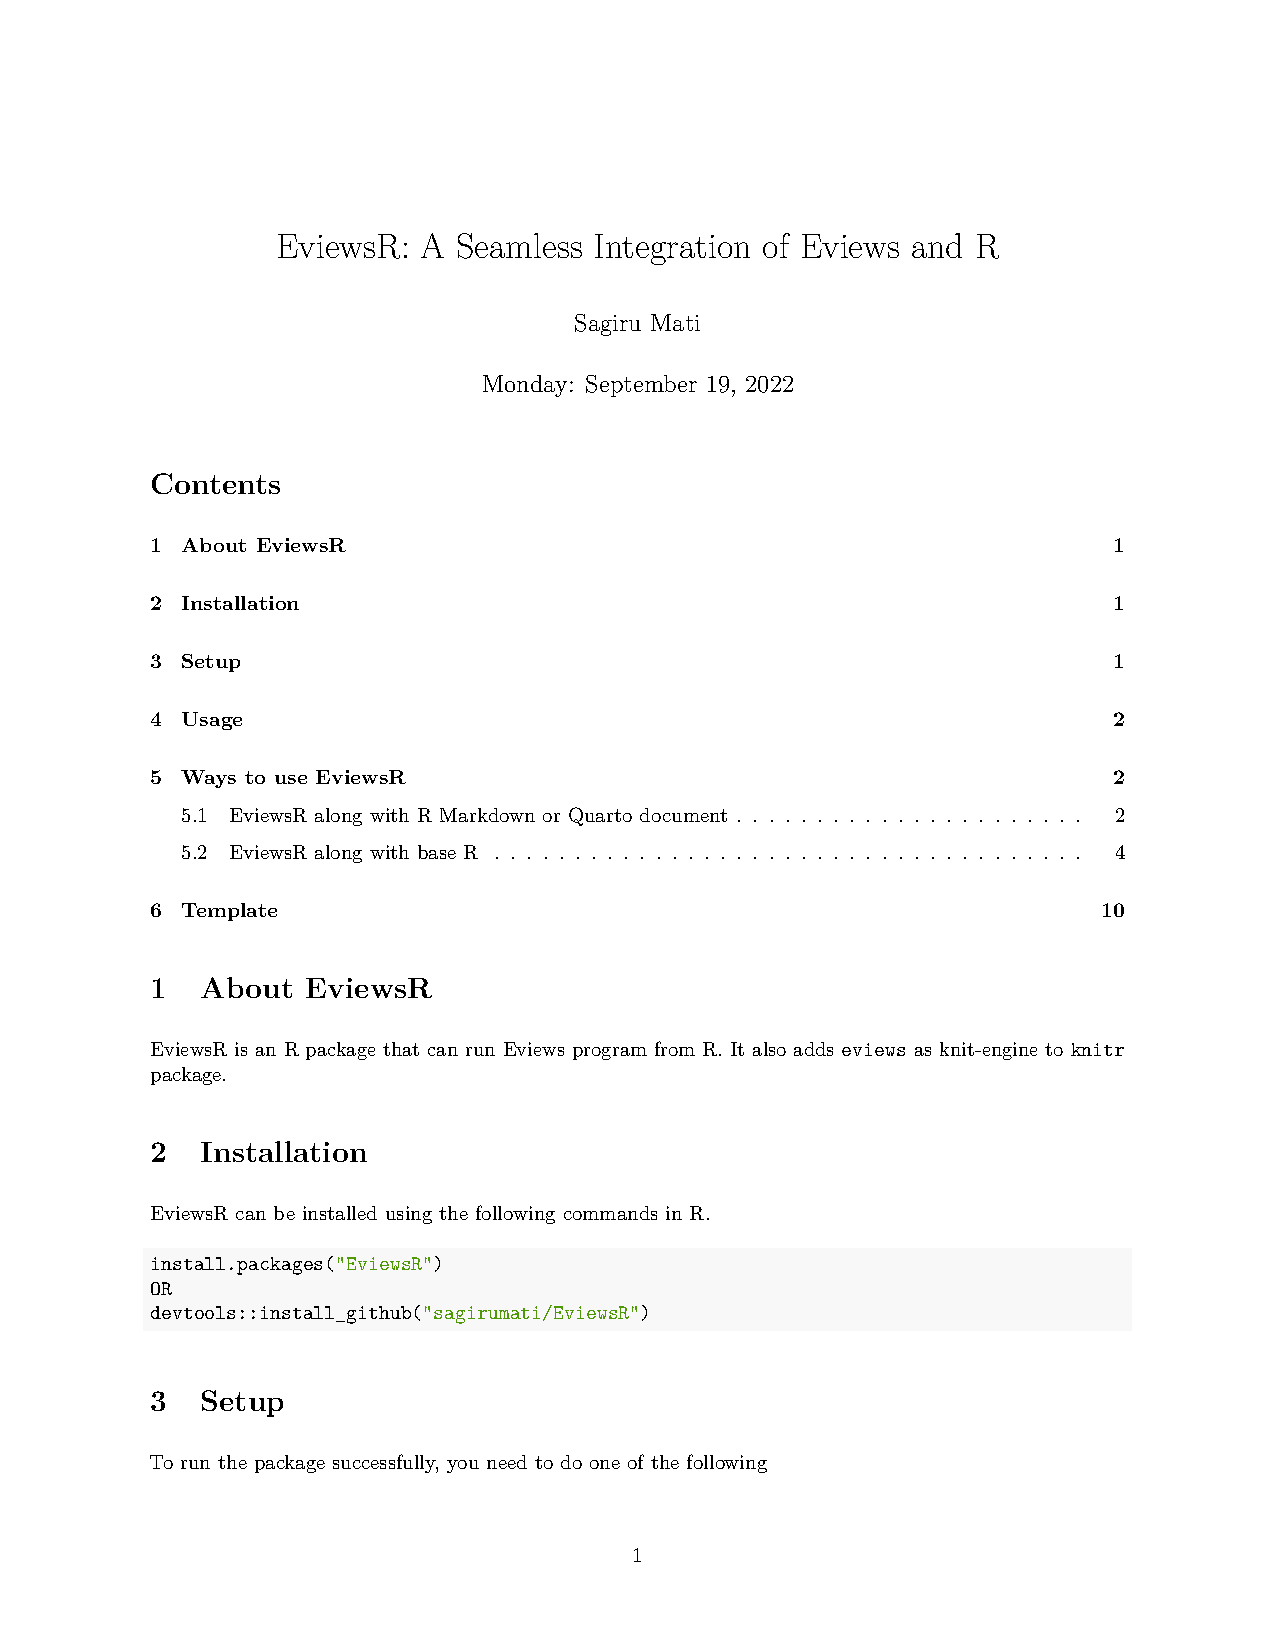
\includegraphics{https://www.r-pkg.org/badges/version/EviewsR.pdf}}
\href{https://cranlogs.r-pkg.org/badges/grand-total/EviewsR?color=49C31B}{\includegraphics{https://cranlogs.r-pkg.org/badges/grand-total/EviewsR?color=49C31B.pdf}}
\href{https://cranlogs.r-pkg.org/badges/EviewsR?color=49C31B}{\includegraphics{https://cranlogs.r-pkg.org/badges/EviewsR?color=49C31B.pdf}}

\hypertarget{about-the-author}{%
\section{About the Author}\label{about-the-author}}

The author of this package, \textbf{Sagiru Mati}, obtained his PhD in
Economics from the Near East University, North Cyprus. He works at the
Department of Economics, Yusuf Maitama Sule (Northwest) University,
Kano, Nigeria. Please visit his \href{https://smati.com.ng}{website} for
more details.

Please follow his publications on \textbf{ORCID: 0000-0003-1413-3974}

\hypertarget{about-eviewsr}{%
\section{About EviewsR}\label{about-eviewsr}}

EviewsR is an R package that can run EViews program in R. It also adds
\texttt{eviews} as a knit-engine to \texttt{knitr} package, so that
users can embed EViews codes in R Markdown and Quarto document.

\hypertarget{installation}{%
\section{Installation}\label{installation}}

EviewsR can be installed using the following commands in R.

\begin{Shaded}
\begin{Highlighting}[]
\FunctionTok{install.packages}\NormalTok{(}\StringTok{"EviewsR"}\NormalTok{)}
\NormalTok{OR}
\NormalTok{devtools}\SpecialCharTok{::}\FunctionTok{install\_github}\NormalTok{(}\StringTok{"sagirumati/EviewsR"}\NormalTok{)}
\end{Highlighting}
\end{Shaded}

\begin{figure}

\end{figure}

\hypertarget{setup}{%
\section{Setup}\label{setup}}

To run the package successfully, you need to do one of the following

\begin{itemize}
\item
  Don't do anything if the name of EViews executable is one of the
  following: \texttt{EViews13\_x64},
  \texttt{EViews13\_x86},\texttt{EViews12\_x64}, \texttt{EViews12\_x86},
  \texttt{EViews11\_x64}, \texttt{EViews11\_x86},\texttt{EViews10\_x64},
  \texttt{EViews10\_x86},\texttt{EViews9\_x64}, \texttt{EViews9\_x86},
  \texttt{EViews10}. The package will find the executable automatically.
\item
  Rename the Eviews executable to \texttt{eviews} or one of the names
  above.
\item
  Alternatively, you can use \texttt{set\_eviews\_path} function to set
  the path the EViews executable as follows:
\end{itemize}

\begin{Shaded}
\begin{Highlighting}[]
\FunctionTok{set\_eviews\_path}\NormalTok{(}\StringTok{"C:/Program Files (x86)/EViews 10/EViews10.exe"}\NormalTok{)}
\end{Highlighting}
\end{Shaded}

\begin{figure}

\end{figure}

\hypertarget{usage}{%
\section{Usage}\label{usage}}

Please load the EviewsR package as follows:

\begin{verbatim}
```{r}                                                                .
library(EviewsR)
```
\end{verbatim}

\hypertarget{ways-to-use-eviewsr}{%
\section{Ways to use EviewsR}\label{ways-to-use-eviewsr}}

The package can work with base R, R Markdown or Quarto document.

\hypertarget{eviewsr-along-with-r-markdown-or-quarto-document}{%
\subsection{EviewsR along with R Markdown or Quarto
document}\label{eviewsr-along-with-r-markdown-or-quarto-document}}

After loading the package, a chunk for Eviews can be created by
supplying \texttt{eviews} as the engine name in R Markdown or Quarto
document as shown below :

\begin{verbatim}
```{eviews} 
#| label: fig-EviewsR
#| eval: true
#| fig.subcap: ["X graph","Y graph"]
#| fig.cap: "EViews graphs imported automatically by fig-EviewsR chunk"

    'This program is created in R Markdown with the help of EviewsR package
  
  wfcreate(page=EviewsRPage,wf=EviewsR_workfile) m 2000 2022
  for %y EviewsR package page1 page2
  pagecreate(page={%y}) EviewsR m 2000 2022
  next
  pageselect EviewsRPage
  rndseed 123456
  genr y=@cumsum(nrnd)
  genr x=@cumsum(nrnd)
  equation ols.ls y c x
  freeze(OLSTable,mode=overwrite) ols
  freeze(EviewsR_Plot,mode=overwrite) y.line
  wfsave EviewsR_workfile
```  
\end{verbatim}

\begin{figure}

\begin{minipage}[t]{0.50\linewidth}

{\centering 

\raisebox{-\height}{

\includegraphics{README_files/figure-pdf//EviewsREviewsRPage-XX.pdf}

}

}

\subcaption{\label{fig-EviewsR-1}X graph}
\end{minipage}%
%
\begin{minipage}[t]{0.50\linewidth}

{\centering 

\raisebox{-\height}{

\includegraphics{README_files/figure-pdf//EviewsREviewsRPage-YY.pdf}

}

}

\subcaption{\label{fig-EviewsR-2}Y graph}
\end{minipage}%

\caption{\label{fig-EviewsR}EViews graphs imported automatically by
fig-EviewsR chunk}

\end{figure}

The above chunk creates an Eviews program with the chunk's content, then
automatically open Eviews and run the program, which will create an
Eviews workfile with pages containing monthly sample from 2000 to 2022.
The program will also save an EViews workfile named
\texttt{EviewsR\_workfile} in the current directory.

The \texttt{eviews} chunk automatically returns the outputs of each
equation object as a dataframe, accessible via
\texttt{chunkLabel\$pageName\_equationName}. For example, The \(R^2\) of
the \texttt{ols} equation object is 0.044951, which can be accessed
using
\texttt{\textasciigrave{}r\ EviewsR\$eviewsrpage\_ols\$r2\textasciigrave{}}.
We can obtain the table object by
\texttt{chunkLabel\$pageName\_tableName}. Therefore,
\texttt{EviewsR\$eviewsrpage\_olstable} will give us the
\texttt{OLSTable} object as dataframe. Note the underscore (\texttt{\_})
between the \texttt{pageName} and \texttt{equationName}, and between the
\texttt{pageName} and \texttt{tableName}.

\begin{Shaded}
\begin{Highlighting}[]
\NormalTok{EviewsR}\SpecialCharTok{$}\NormalTok{eviewsrpage\_ols}\SpecialCharTok{$}\NormalTok{r2}
\CommentTok{\#\textgreater{} [1] 0.044951}
\NormalTok{EviewsR}\SpecialCharTok{$}\NormalTok{eviewsrpage\_ols}\SpecialCharTok{$}\NormalTok{aic}
\CommentTok{\#\textgreater{} [1] 4.310163}
\NormalTok{K }\OtherTok{=}\NormalTok{ EviewsR}\SpecialCharTok{$}\NormalTok{eviewsrpage\_olstable[}\FunctionTok{c}\NormalTok{(}\DecValTok{6}\NormalTok{, }\DecValTok{8}\NormalTok{, }\DecValTok{9}\NormalTok{), }\DecValTok{1}\SpecialCharTok{:}\DecValTok{5}\NormalTok{]}
\FunctionTok{colnames}\NormalTok{(K) }\OtherTok{=} \ConstantTok{NULL}
\NormalTok{knitr}\SpecialCharTok{::}\FunctionTok{kable}\NormalTok{(K, }\AttributeTok{row.names =}\NormalTok{ F, }\AttributeTok{caption =} \StringTok{"Selected cells of  EViews table object"}\NormalTok{)}
\end{Highlighting}
\end{Shaded}

\begin{figure}

\begin{minipage}[t]{0.50\linewidth}

{\centering 

\begin{longtable}[]{@{}lllll@{}}
\caption{Selected cells of EViews table object}\tabularnewline
\toprule()
\endhead
Variable & Coefficient & Std. Error & t-Statistic & Prob. \\
C & -0.301413 & 0.260956 & -1.155033 & 0.2491 \\
X & -0.051410 & 0.014316 & -3.591137 & 0.0004 \\
\bottomrule()
\end{longtable}

}

\end{minipage}%

\end{figure}

The EViews series objects are also imported automatically as dataframe
(by default) or \texttt{xts} objects (if we use chunk option
\texttt{class="xts"}). They are accessed via
\texttt{chunkLabel\$pageName}.

\begin{Shaded}
\begin{Highlighting}[]
\NormalTok{EviewsR}\SpecialCharTok{$}\NormalTok{eviewsrpage }\SpecialCharTok{|\textgreater{}}
    \FunctionTok{head}\NormalTok{()}
\CommentTok{\#\textgreater{}         date           x          y}
\CommentTok{\#\textgreater{} 1 2000{-}01{-}01 {-}0.06062345 0.34705763}
\CommentTok{\#\textgreater{} 2 2000{-}02{-}01  0.40287977 0.04959103}
\CommentTok{\#\textgreater{} 3 2000{-}03{-}01  1.13387526 0.56589164}
\CommentTok{\#\textgreater{} 4 2000{-}04{-}01  1.34089330 1.35264827}
\CommentTok{\#\textgreater{} 5 2000{-}05{-}01  0.54596099 1.05434874}
\CommentTok{\#\textgreater{} 6 2000{-}06{-}01  0.96869514 0.61693341}
\end{Highlighting}
\end{Shaded}

\begin{figure}

\end{figure}

\hypertarget{eviewsr-along-with-base-r}{%
\subsection{EviewsR along with base R}\label{eviewsr-along-with-base-r}}

\hypertarget{the-create_object-function}{%
\subsubsection{The create\_object()
function}\label{the-create_object-function}}

The function \texttt{create\_object()} can be used to create an Eviews
object in the existing EViews workfile.

\begin{Shaded}
\begin{Highlighting}[]
\FunctionTok{create\_object}\NormalTok{(}\AttributeTok{wf =} \StringTok{"EviewsR\_workfile"}\NormalTok{, }\AttributeTok{action =} \StringTok{"equation"}\NormalTok{, }\AttributeTok{action\_opt =} \StringTok{""}\NormalTok{,}
    \AttributeTok{object\_name =} \StringTok{"eviews\_equation"}\NormalTok{, }\AttributeTok{view\_or\_proc =} \StringTok{"ls"}\NormalTok{, }\AttributeTok{options\_list =} \StringTok{""}\NormalTok{,}
    \AttributeTok{arg\_list =} \StringTok{"y ar(1)"}\NormalTok{)}
\end{Highlighting}
\end{Shaded}

\begin{figure}

\end{figure}

\begin{Shaded}
\begin{Highlighting}[]
\FunctionTok{create\_object}\NormalTok{(}\AttributeTok{wf =} \StringTok{"EviewsR\_workfile"}\NormalTok{, }\AttributeTok{object\_name =} \StringTok{"x1"}\NormalTok{, }\AttributeTok{object\_type =} \StringTok{"series"}\NormalTok{,}
    \AttributeTok{expression =} \StringTok{"y\^{}2"}\NormalTok{)}
\end{Highlighting}
\end{Shaded}

\begin{figure}

\end{figure}

\hypertarget{the-eviews_graph-function}{%
\subsubsection{The eviews\_graph()
function}\label{the-eviews_graph-function}}

EViews graphs can be included in R Markdown or Quarto document by
\texttt{eviews\_graph()} function.

To create graph from existing EViews series objects:

\begin{Shaded}
\begin{Highlighting}[]
\FunctionTok{eviews\_graph}\NormalTok{(}\AttributeTok{wf =} \StringTok{"EviewsR\_workfile"}\NormalTok{, }\AttributeTok{page =} \StringTok{"EviewsRPage"}\NormalTok{, }\AttributeTok{series =} \StringTok{"x y"}\NormalTok{,}
    \AttributeTok{mode =} \StringTok{"overwrite"}\NormalTok{, }\AttributeTok{graph\_options =} \StringTok{"m"}\NormalTok{)}
\end{Highlighting}
\end{Shaded}

\begin{figure}

\begin{minipage}[t]{0.50\linewidth}

{\centering 

\raisebox{-\height}{

\includegraphics{README_files/figure-pdf//eviewsGraph-EviewsRPage-X.pdf}

}

\caption{\label{fig-eviewsGraph-1}Graphs of existing EViews series
objects imported by fig-eviewsGraph chunk}

}

\end{minipage}%
%
\begin{minipage}[t]{0.50\linewidth}

{\centering 

\raisebox{-\height}{

\includegraphics{README_files/figure-pdf//eviewsGraph-EviewsRPage-Y.pdf}

}

\caption{\label{fig-eviewsGraph-2}Graphs of existing EViews series
objects imported by fig-eviewsGraph chunk}

}

\end{minipage}%

\end{figure}

We can also create objects from an R dataframe

\begin{Shaded}
\begin{Highlighting}[]
\NormalTok{Data }\OtherTok{=} \FunctionTok{data.frame}\NormalTok{(}\AttributeTok{x =} \FunctionTok{cumsum}\NormalTok{(}\FunctionTok{rnorm}\NormalTok{(}\DecValTok{100}\NormalTok{)), }\AttributeTok{y =} \FunctionTok{cumsum}\NormalTok{(}\FunctionTok{rnorm}\NormalTok{(}\DecValTok{100}\NormalTok{)))}
\FunctionTok{eviews\_graph}\NormalTok{(}\AttributeTok{series =}\NormalTok{ Data, }\AttributeTok{group =} \ConstantTok{TRUE}\NormalTok{, }\AttributeTok{start\_date =} \StringTok{"1990Q4"}\NormalTok{,}
    \AttributeTok{frequency =} \StringTok{"Q"}\NormalTok{)}
\end{Highlighting}
\end{Shaded}

\begin{figure}

\begin{minipage}[t]{0.50\linewidth}

{\centering 

\raisebox{-\height}{

\includegraphics{README_files/figure-pdf//eviewsGraph1-Eviewsgraph1-XY.pdf}

}

\caption{\label{fig-eviewsGraph1}Graphs of an R dataframe imported by
fig-eviewsGraph1 chunk}

}

\end{minipage}%

\end{figure}

\hypertarget{the-eviews_import-function}{%
\subsubsection{The eviews\_import()
function}\label{the-eviews_import-function}}

Data can be imported from external sources by \texttt{eviews\_import()}
function.

\begin{figure}

\end{figure}

\begin{Shaded}
\begin{Highlighting}[]
\FunctionTok{eviews\_import}\NormalTok{(}\AttributeTok{source\_description =} \StringTok{"eviews\_import.csv"}\NormalTok{, }\AttributeTok{start\_date =} \StringTok{"1990"}\NormalTok{,}
    \AttributeTok{frequency =} \StringTok{"m"}\NormalTok{, }\AttributeTok{rename\_string =} \StringTok{"x ab"}\NormalTok{, }\AttributeTok{smpl\_string =} \StringTok{"1990m10 1992m10"}\NormalTok{)}
\end{Highlighting}
\end{Shaded}

\begin{figure}

\end{figure}

Alternatively, use the dataframe as the \texttt{source\_description}.

\begin{Shaded}
\begin{Highlighting}[]
\FunctionTok{eviews\_import}\NormalTok{(}\AttributeTok{source\_description =}\NormalTok{ Data, }\AttributeTok{wf =} \StringTok{"eviews\_import1"}\NormalTok{,}
    \AttributeTok{start\_date =} \StringTok{"1990"}\NormalTok{, }\AttributeTok{frequency =} \StringTok{"m"}\NormalTok{, }\AttributeTok{rename\_string =} \StringTok{"x ab"}\NormalTok{,}
    \AttributeTok{smpl\_string =} \StringTok{"1990m10 1992m10"}\NormalTok{)}
\end{Highlighting}
\end{Shaded}

\begin{figure}

\end{figure}

\hypertarget{the-eviews_pagesave-function}{%
\subsubsection{The eviews\_pagesave()
function}\label{the-eviews_pagesave-function}}

Similar to Eviews workfile, an Eviews page can be saved in various
formats by \texttt{eviews\_pagesave()} function.

\begin{Shaded}
\begin{Highlighting}[]
\FunctionTok{eviews\_pagesave}\NormalTok{(}\AttributeTok{wf =} \StringTok{"eviewsr\_workfile"}\NormalTok{, }\AttributeTok{page =} \StringTok{"EviewsRPage"}\NormalTok{,}
    \AttributeTok{source\_description =} \StringTok{"pagesave.csv"}\NormalTok{, }\AttributeTok{drop\_list =} \StringTok{"y"}\NormalTok{)}
\end{Highlighting}
\end{Shaded}

\begin{figure}

\end{figure}

\hypertarget{the-eviews_wfcreate-function}{%
\subsubsection{The eviews\_wfcreate()
function}\label{the-eviews_wfcreate-function}}

An Eviews workfile can be created using \texttt{eviews\_wfcreate()}
function in R.

\begin{Shaded}
\begin{Highlighting}[]
\FunctionTok{eviews\_wfcreate}\NormalTok{(}\AttributeTok{wf =} \StringTok{"eviews\_wfcreate"}\NormalTok{, }\AttributeTok{page =} \StringTok{"EviewsRPage"}\NormalTok{,}
    \AttributeTok{frequency =} \StringTok{"m"}\NormalTok{, }\AttributeTok{start\_date =} \StringTok{"1990"}\NormalTok{, }\AttributeTok{end\_date =} \StringTok{"2022"}\NormalTok{)}
\end{Highlighting}
\end{Shaded}

\begin{figure}

\end{figure}

Create a workfile from a dataframe

\begin{Shaded}
\begin{Highlighting}[]
\FunctionTok{eviews\_wfcreate}\NormalTok{(}\AttributeTok{source\_description =}\NormalTok{ Data, }\AttributeTok{wf =} \StringTok{"eviews\_wfcreate1"}\NormalTok{,}
    \AttributeTok{page =} \StringTok{"EviewsR\_page"}\NormalTok{, }\AttributeTok{frequency =} \StringTok{"m"}\NormalTok{, }\AttributeTok{start\_date =} \StringTok{"1990"}\NormalTok{)}
\end{Highlighting}
\end{Shaded}

\begin{figure}

\end{figure}

\hypertarget{the-eviews_wfsave-function}{%
\subsubsection{The eviews\_wfsave()
function}\label{the-eviews_wfsave-function}}

An EViews workfile can be saved various output formats using
\texttt{eviews\_wfsave()} in function in R.

\begin{Shaded}
\begin{Highlighting}[]
\FunctionTok{eviews\_wfsave}\NormalTok{(}\AttributeTok{wf =} \StringTok{"eviewsr\_workfile"}\NormalTok{, }\AttributeTok{source\_description =} \StringTok{"wfsave.csv"}\NormalTok{)}
\end{Highlighting}
\end{Shaded}

\begin{figure}

\end{figure}

\hypertarget{the-exec_commands-function}{%
\subsubsection{The exec\_commands()
function}\label{the-exec_commands-function}}

A set of Eviews commands can be executed with the help of
\texttt{exec\_commands()} function in R.

\begin{Shaded}
\begin{Highlighting}[]
\FunctionTok{exec\_commands}\NormalTok{(}\FunctionTok{c}\NormalTok{(}\StringTok{"wfcreate(wf=exec\_commands,page=eviewsPage) m 2000 2022"}\NormalTok{))}
\end{Highlighting}
\end{Shaded}

\begin{figure}

\end{figure}

\begin{Shaded}
\begin{Highlighting}[]
\NormalTok{eviewsCommands }\OtherTok{=} \StringTok{"pagecreate(page=eviewspage1) 7 2020 2022}
\StringTok{for \%page eviewspage eviewspage1}
\StringTok{pageselect \{\%page\}}
\StringTok{genr y=@cumsum(nrnd)}
\StringTok{genr x=@cumsum(nrnd)}
\StringTok{equation ols.ls y c x}
\StringTok{graph x\_graph.line x}
\StringTok{graph y\_graph.area y}
\StringTok{freeze(OLSTable,mode=overwrite) ols}
\StringTok{next}
\StringTok{"}
\FunctionTok{exec\_commands}\NormalTok{(}\AttributeTok{commands =}\NormalTok{ eviewsCommands, }\AttributeTok{wf =} \StringTok{"exec\_commands"}\NormalTok{)}
\end{Highlighting}
\end{Shaded}

\begin{figure}

\end{figure}

\hypertarget{the-export_dataframe-function}{%
\subsubsection{The export\_dataframe()
function}\label{the-export_dataframe-function}}

Use \texttt{export\_dataframe()} function to export dataframe object to
Eviews.

\begin{Shaded}
\begin{Highlighting}[]
\FunctionTok{export\_dataframe}\NormalTok{(}\AttributeTok{wf =} \StringTok{"export\_dataframe"}\NormalTok{, }\AttributeTok{source\_description =}\NormalTok{ Data,}
    \AttributeTok{start\_date =} \StringTok{"1990"}\NormalTok{, }\AttributeTok{frequency =} \StringTok{"m"}\NormalTok{)}
\end{Highlighting}
\end{Shaded}

\begin{figure}

\end{figure}

\hypertarget{the-import_equation-function}{%
\subsubsection{The import\_equation()
function}\label{the-import_equation-function}}

Import EViews equation data members into R, R Markdown or Quarto.

\begin{Shaded}
\begin{Highlighting}[]
\FunctionTok{import\_equation}\NormalTok{(}\AttributeTok{wf =} \StringTok{"EviewsR\_workfile"}\NormalTok{, }\AttributeTok{page =} \StringTok{"EviewsRPage"}\NormalTok{,}
    \AttributeTok{equation =} \StringTok{"OLS"}\NormalTok{)}
\end{Highlighting}
\end{Shaded}

\begin{figure}

\end{figure}

To access the imported equation in base R:

\begin{figure}

\end{figure}

\hypertarget{the-import_graph-function}{%
\subsubsection{The import\_graph()
function}\label{the-import_graph-function}}

Import EViews graph objects(s) into R, R Markdown or Quarto.

\begin{Shaded}
\begin{Highlighting}[]
\FunctionTok{import\_graph}\NormalTok{(}\AttributeTok{wf =} \StringTok{"eviewsr\_workfile"}\NormalTok{)}
\end{Highlighting}
\end{Shaded}

\begin{figure}

\begin{minipage}[t]{0.50\linewidth}

{\centering 

\raisebox{-\height}{

\includegraphics{README_files/figure-pdf//fig-importGraph-EviewsRPage-XX.pdf}

}

\caption{\label{fig-importGraph-1}EViews graphs imported using
import\_graph() function}

}

\end{minipage}%
%
\begin{minipage}[t]{0.50\linewidth}

{\centering 

\raisebox{-\height}{

\includegraphics{README_files/figure-pdf//fig-importGraph-EviewsRPage-YY.pdf}

}

\caption{\label{fig-importGraph-2}EViews graphs imported using
import\_graph() function}

}

\end{minipage}%

\end{figure}

To import only graphs that begin with x:

\begin{Shaded}
\begin{Highlighting}[]
\FunctionTok{import\_graph}\NormalTok{(}\AttributeTok{wf =} \StringTok{"exec\_commands"}\NormalTok{, }\AttributeTok{graph =} \StringTok{"x*"}\NormalTok{)}
\end{Highlighting}
\end{Shaded}

\begin{figure}

\begin{minipage}[t]{0.50\linewidth}

{\centering 

\raisebox{-\height}{

\includegraphics{README_files/figure-pdf//fig-importGraph1-eviewsPage-X_GRAPH.pdf}

}

\caption{\label{fig-importGraph1-1}EViews graphs that begin with X
imported using import\_graph() function}

}

\end{minipage}%
%
\begin{minipage}[t]{0.50\linewidth}

{\centering 

\raisebox{-\height}{

\includegraphics{README_files/figure-pdf//fig-importGraph1-eviewspage1-X_GRAPH.pdf}

}

\caption{\label{fig-importGraph1-2}EViews graphs that begin with X
imported using import\_graph() function}

}

\end{minipage}%

\end{figure}

\hypertarget{the-import_kable-function}{%
\subsubsection{The import\_kable()
function}\label{the-import_kable-function}}

Eviews tables can be imported as \texttt{kable} object by
\texttt{import\_kable()} function. Therefore, we can include the

\begin{Shaded}
\begin{Highlighting}[]
\FunctionTok{import\_kable}\NormalTok{(}\AttributeTok{wf=}\StringTok{"EViewsR\_workfile"}\NormalTok{,}\AttributeTok{page=}\StringTok{"EviewsRPage"}\NormalTok{,}\AttributeTok{table =} \StringTok{"OLSTable"}\NormalTok{,}
\AttributeTok{caption =} \StringTok{"Selected cells of EViews table imported using import}\SpecialCharTok{\textbackslash{}\textbackslash{}}\StringTok{\_kable() function"}\NormalTok{,}
\AttributeTok{range =} \StringTok{"r7c1:r10c5"}\NormalTok{,}\AttributeTok{digits=}\DecValTok{3}\NormalTok{)}
\end{Highlighting}
\end{Shaded}

\begin{figure}

\begin{minipage}[t]{0.50\linewidth}

{\centering 

\caption{Selected cells of EViews table imported using import\_kable() function}
\centering
\begin{tabular}[t]{lrrrr}
\toprule
Variable & Coefficient & Std. Error & t-Statistic & Prob.\\
\midrule
C & -0.301 & 0.261 & -1.155 & 0.249\\
X & -0.051 & 0.014 & -3.591 & 0.000\\
\bottomrule
\end{tabular}

}

\end{minipage}%

\end{figure}

\hypertarget{the-import_series-function}{%
\subsubsection{The import\_series()
function}\label{the-import_series-function}}

Use \texttt{import\_series()} function to import data from EViews to R
as a dataframe. The function creates a new environment \texttt{eviews},
whose objects can be accessed via \texttt{eviews\$pageName}.

\begin{Shaded}
\begin{Highlighting}[]
\FunctionTok{import\_series}\NormalTok{(}\AttributeTok{wf =} \StringTok{"eviewsr\_workfile"}\NormalTok{)}
\end{Highlighting}
\end{Shaded}

\begin{figure}

\end{figure}

To access the series in base R:

\begin{Shaded}
\begin{Highlighting}[]
\NormalTok{eviews}\SpecialCharTok{$}\NormalTok{eviewspage }\SpecialCharTok{|\textgreater{}}
    \FunctionTok{head}\NormalTok{()}
\end{Highlighting}
\end{Shaded}

\begin{figure}

\end{figure}

To import the series as an \texttt{xts} object:

\begin{Shaded}
\begin{Highlighting}[]
\FunctionTok{import\_series}\NormalTok{(}\AttributeTok{wf =} \StringTok{"eviewsr\_workfile"}\NormalTok{, }\AttributeTok{series =} \FunctionTok{c}\NormalTok{(}\StringTok{"x"}\NormalTok{, }\StringTok{"y"}\NormalTok{),}
    \AttributeTok{class =} \StringTok{"xts"}\NormalTok{)}
\end{Highlighting}
\end{Shaded}

\begin{figure}

\end{figure}

\hypertarget{the-import_table-function}{%
\subsubsection{The import\_table()
function}\label{the-import_table-function}}

Import EViews table objects(s) into R, R Markdown or Quarto.

To import all table objects across all pages

\begin{Shaded}
\begin{Highlighting}[]
\FunctionTok{import\_table}\NormalTok{(}\AttributeTok{wf =} \StringTok{"EviewsR\_workfile"}\NormalTok{)}
\end{Highlighting}
\end{Shaded}

\begin{figure}

\end{figure}

To import specific table objects, for example \texttt{OLSTable}

\begin{Shaded}
\begin{Highlighting}[]
\FunctionTok{import\_table}\NormalTok{(}\AttributeTok{wf =} \StringTok{"EviewsR\_workfile"}\NormalTok{, }\AttributeTok{table =} \StringTok{"OLStable"}\NormalTok{)}
\end{Highlighting}
\end{Shaded}

\begin{figure}

\end{figure}

To import table objects on specific pages

\begin{Shaded}
\begin{Highlighting}[]
\FunctionTok{import\_table}\NormalTok{(}\AttributeTok{wf =} \StringTok{"EviewsR\_workfile"}\NormalTok{, }\AttributeTok{page =} \StringTok{" EviewsRPage"}\NormalTok{)}
\end{Highlighting}
\end{Shaded}

\begin{figure}

\end{figure}

To access the table in base R (\texttt{eviews\$pageName\_tableName})

\begin{Shaded}
\begin{Highlighting}[]
\NormalTok{eviews}\SpecialCharTok{$}\NormalTok{eviewspage\_olstable}
\end{Highlighting}
\end{Shaded}

\begin{figure}

\end{figure}

\hypertarget{the-import_workfile-function}{%
\subsubsection{The import\_workfile()
function}\label{the-import_workfile-function}}

Import EViews equation data members, graph, series and table objects(s)
into R, R Markdown or Quarto.

To import all equation, graph, series and table objects across all pages

\begin{Shaded}
\begin{Highlighting}[]
\FunctionTok{import\_workfile}\NormalTok{(}\AttributeTok{wf =} \StringTok{"EviewsR\_workfile"}\NormalTok{)}
\end{Highlighting}
\end{Shaded}

\begin{figure}

\begin{minipage}[t]{0.50\linewidth}

{\centering 

\raisebox{-\height}{

\includegraphics{README_files/figure-pdf//fig-importWorkfile-EviewsRPage-XX.pdf}

}

\caption{\label{fig-importWorkfile-1}EViews graphs automatically
imported by import\_workfile() function}

}

\end{minipage}%
%
\begin{minipage}[t]{0.50\linewidth}

{\centering 

\raisebox{-\height}{

\includegraphics{README_files/figure-pdf//fig-importWorkfile-EviewsRPage-YY.pdf}

}

\caption{\label{fig-importWorkfile-2}EViews graphs automatically
imported by import\_workfile() function}

}

\end{minipage}%

\end{figure}

To import specific objects

\begin{Shaded}
\begin{Highlighting}[]
\FunctionTok{import\_workfile}\NormalTok{(}\AttributeTok{wf =} \StringTok{"exec\_commands"}\NormalTok{, }\AttributeTok{equation =} \StringTok{"ols"}\NormalTok{, }\AttributeTok{graph =} \StringTok{"x*"}\NormalTok{,}
    \AttributeTok{series =} \StringTok{"y*"}\NormalTok{, }\AttributeTok{table =} \StringTok{"ols*"}\NormalTok{)}
\end{Highlighting}
\end{Shaded}

\begin{figure}

\end{figure}

To import objects on specific page(s)

\begin{Shaded}
\begin{Highlighting}[]
\FunctionTok{import\_workfile}\NormalTok{(}\AttributeTok{wf =} \StringTok{"exec\_commands"}\NormalTok{, }\AttributeTok{page =} \StringTok{"eviewspage eviewspage1"}\NormalTok{)}
\end{Highlighting}
\end{Shaded}

\begin{figure}

\end{figure}

\hypertarget{the-rwalk-function}{%
\subsubsection{The rwalk() function}\label{the-rwalk-function}}

A set of random walk series can be simulated in R using EViews engine,
thanks to \texttt{rwalk()} function.

\begin{Shaded}
\begin{Highlighting}[]
\FunctionTok{rwalk}\NormalTok{(}\AttributeTok{wf =} \StringTok{"eviewsr\_workfile"}\NormalTok{, }\AttributeTok{series =} \StringTok{"X Y Z"}\NormalTok{, }\AttributeTok{page =} \StringTok{""}\NormalTok{, }\AttributeTok{rndseed =} \DecValTok{12345}\NormalTok{,}
    \AttributeTok{frequency =} \StringTok{"M"}\NormalTok{, }\AttributeTok{num\_observations =} \DecValTok{100}\NormalTok{, }\AttributeTok{class =} \StringTok{"xts"}\NormalTok{)}
\end{Highlighting}
\end{Shaded}

\begin{figure}

\end{figure}

\begin{Shaded}
\begin{Highlighting}[]
\NormalTok{xts}\SpecialCharTok{::}\FunctionTok{plot.xts}\NormalTok{(rwalk}\SpecialCharTok{$}\NormalTok{xyz, }\AttributeTok{type =} \StringTok{"l"}\NormalTok{, }\AttributeTok{main =} \StringTok{""}\NormalTok{)}
\NormalTok{ggplot2}\SpecialCharTok{::}\FunctionTok{autoplot}\NormalTok{(rwalk}\SpecialCharTok{$}\NormalTok{xyz, }\AttributeTok{facet =} \StringTok{""}\NormalTok{)}
\end{Highlighting}
\end{Shaded}

\begin{figure}

\begin{minipage}[t]{0.50\linewidth}

{\centering 

\raisebox{-\height}{

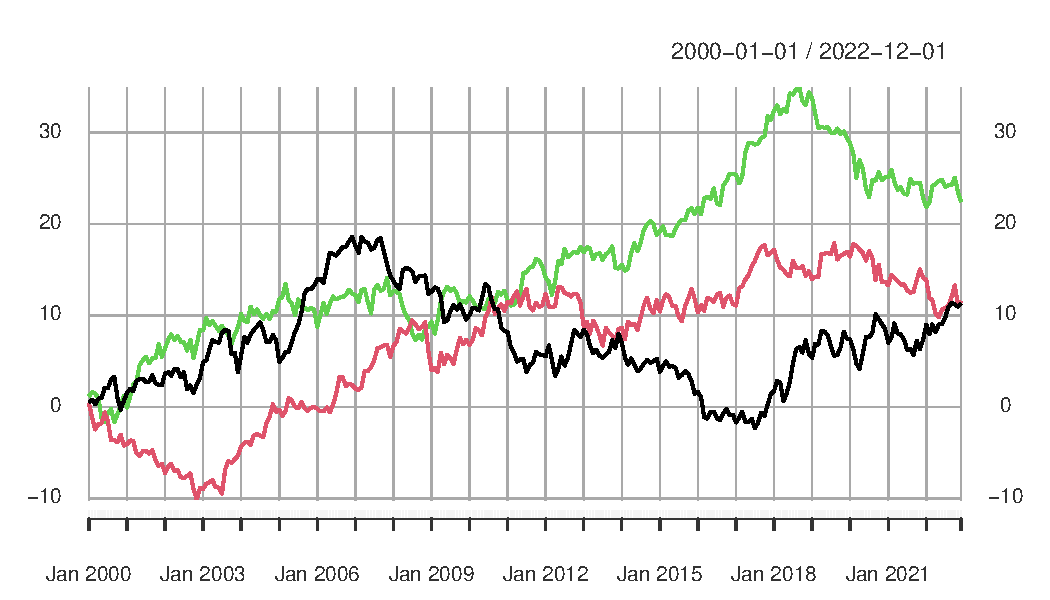
\includegraphics{README_files/figure-pdf/fig-rwalk-1.pdf}

}

\caption{\label{fig-rwalk-1}Plots of imported EViews random walk series
objects}

}

\end{minipage}%
%
\begin{minipage}[t]{0.50\linewidth}

{\centering 

\raisebox{-\height}{

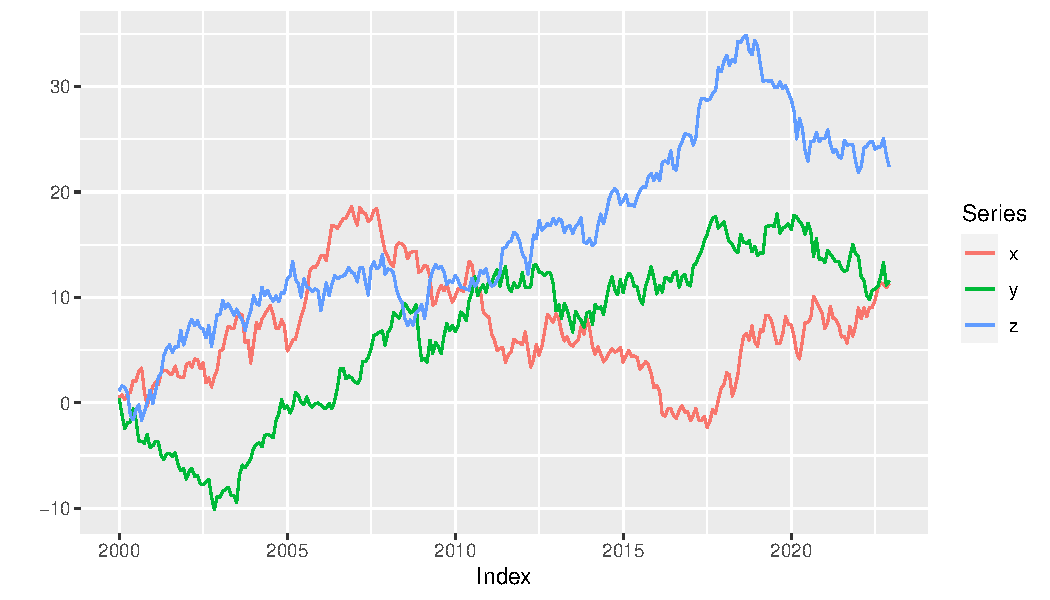
\includegraphics{README_files/figure-pdf/fig-rwalk-2.pdf}

}

\caption{\label{fig-rwalk-2}Plots of imported EViews random walk series
objects}

}

\end{minipage}%

\end{figure}

\hypertarget{demo}{%
\subsubsection{Demo}\label{demo}}

The demo files are included and can be accessed via
\texttt{demo(package="EviewsR")}

\begin{Shaded}
\begin{Highlighting}[]
\FunctionTok{demo}\NormalTok{(}\FunctionTok{create\_object}\NormalTok{())}
\FunctionTok{demo}\NormalTok{(}\FunctionTok{eviews\_graph}\NormalTok{())}
\FunctionTok{demo}\NormalTok{(}\FunctionTok{eviews\_import}\NormalTok{())}
\FunctionTok{demo}\NormalTok{(}\FunctionTok{eviews\_pagesave}\NormalTok{())}
\FunctionTok{demo}\NormalTok{(}\FunctionTok{eviews\_wfcreate}\NormalTok{())}
\FunctionTok{demo}\NormalTok{(}\FunctionTok{eviews\_wfsave}\NormalTok{())}
\FunctionTok{demo}\NormalTok{(}\FunctionTok{exec\_commands}\NormalTok{())}
\FunctionTok{demo}\NormalTok{(}\FunctionTok{export\_dataframe}\NormalTok{())}
\FunctionTok{demo}\NormalTok{(}\FunctionTok{import\_equation}\NormalTok{())}
\FunctionTok{demo}\NormalTok{(}\FunctionTok{import\_graph}\NormalTok{())}
\FunctionTok{demo}\NormalTok{(}\FunctionTok{import\_kable}\NormalTok{())}
\FunctionTok{demo}\NormalTok{(}\FunctionTok{import\_series}\NormalTok{())}
\FunctionTok{demo}\NormalTok{(}\FunctionTok{import\_table}\NormalTok{())}
\FunctionTok{demo}\NormalTok{(}\FunctionTok{import\_workfile}\NormalTok{())}
\FunctionTok{demo}\NormalTok{(}\FunctionTok{rwalk}\NormalTok{())}
\FunctionTok{demo}\NormalTok{(}\FunctionTok{set\_eviews\_path}\NormalTok{())}
\end{Highlighting}
\end{Shaded}

\begin{figure}

\end{figure}

\hypertarget{template}{%
\section{Template}\label{template}}

Template for R Markdown is created. Go to
\texttt{file-\textgreater{}New\ File-\textgreater{}R\ Markdown-\textgreater{}\ From\ Template-\textgreater{}EviewsR}.

Please download the example files from
\href{https://github.com/sagirumati/EviewsR/tree/master/inst/examples/}{Github}.



\end{document}
